\section{Xilinx ZYNQ-7010 device}\label{sec:xilinx}

The three systems proposed in Section \ref{sec:methodology} were implemented and targeted in the ZYNQ-7010 device to assess the performance of the \ac{HP} ports. Due to the existence of four distinct \ac{HP} ports, multiple \ac{DMA} engines were implemented in the \ac{PL}. The used \ac{DMA} engine was the regular one that comes with Xilinx Vivado 2018.3 since it is capable of fully exploiting the bandwidth of the on-chip high-performance interfaces~\cite{xilinx2019dma}. Additionally, two simple circuits were implemented to absorb the streams exported by the \ac{DMA} engines and to produce streams to be consumed. These two circuits were used in the systems to evaluate the \ac{PS}-to-\ac{PL} and \ac{PL}-to-\ac{PS} bandwidths, respectively. While the circuit implemented to absorb the streams produced by the \ac{DMA} engines consists of a single constant connected the \textit{ready} signal of the AXI4-Stream master interface~\cite{xilinx2011axi}, the circuit to generate data streams is more complex, consisting of a \ac{FSM} that generates a predetermined number of words, one per cycle. The system that evaluates the duplex bandwidth features twice as many \ac{DMA} engines as the other two systems. In that system, the \ac{DMA} engines are paired and connected through a \ac{FIFO}, as shown in Figure~\ref{fig:xilinx_duplex}. Figures \ref{fig:xilinx_ps2pl} and \ref{fig:xilinx_pl2ps} illustrate the architectures of the systems to evaluate the \ac{PS}-to-\ac{PL} and \ac{PL}-to-\ac{PS} bandwidths, respectively.

\begin{figure}[!t]
    \centering
    \begin{subfigure}[m]{\linewidth}
        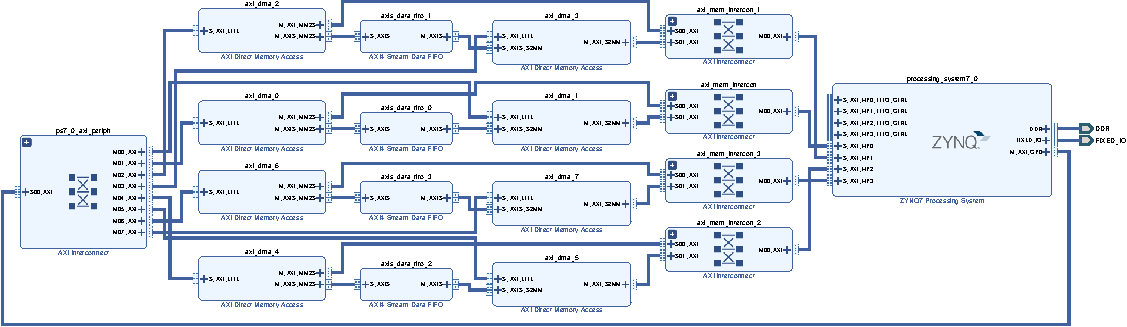
\includegraphics[width=\linewidth]{figures/xilinx_portrait_duplex.pdf}
        \caption{}
        \label{fig:xilinx_duplex}
    \end{subfigure}\\\medskip
    \begin{subfigure}[m]{\linewidth}
        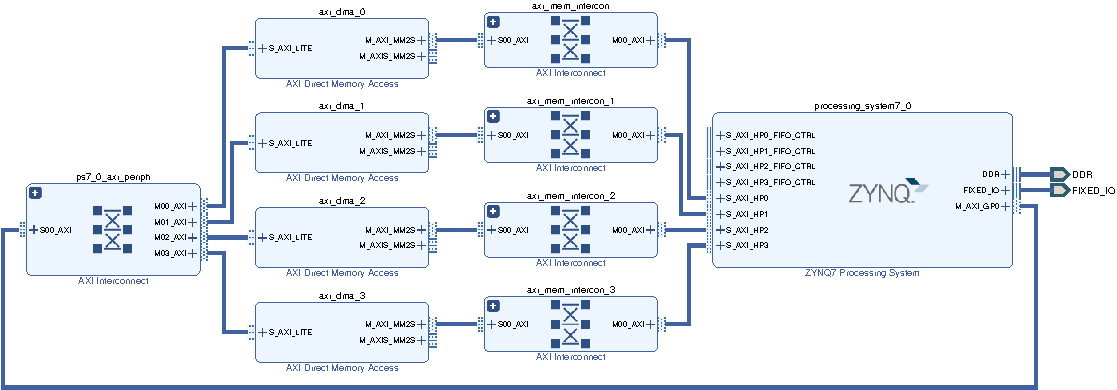
\includegraphics[width=\linewidth]{figures/xilinx_portrait_ps2pl.pdf}
        \caption{}
        \label{fig:xilinx_ps2pl}
    \end{subfigure}\\\medskip
    \begin{subfigure}[m]{\linewidth}
        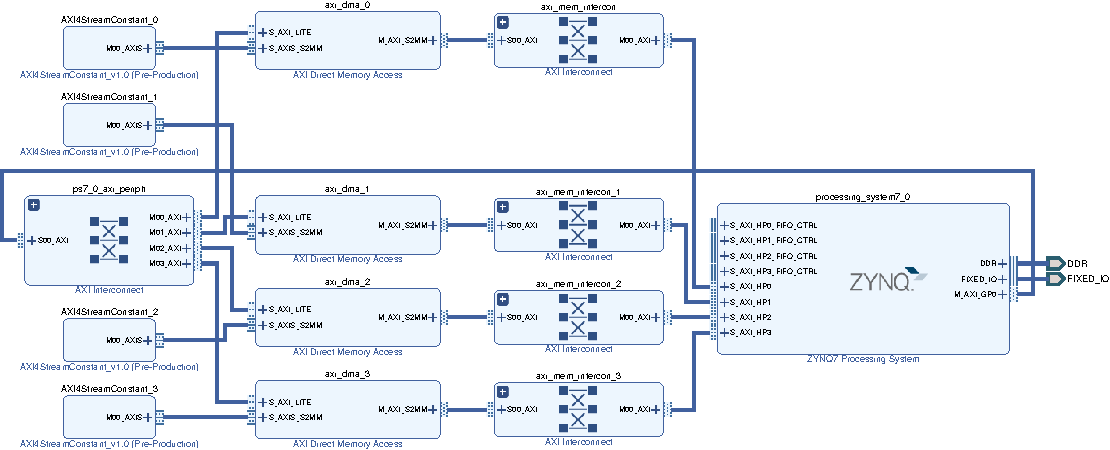
\includegraphics[width=\linewidth]{figures/xilinx_portrait_pl2ps.pdf}
        \caption{}
        \label{fig:xilinx_pl2ps}
    \end{subfigure}
    \caption{Block designs of the systems to evaluate the (\subref{fig:xilinx_duplex}) duplex, (\subref{fig:xilinx_ps2pl}) \ac{PS}-to-\ac{PL}, and (\subref{fig:xilinx_pl2ps}) \ac{PL}-to-\ac{PS} bandwidths of the on-chip high-performance interfaces of the Xilinx device.}
    \label{fig:xilinx_systems}
\end{figure}

To control and monitor the data transfers through the \ac{DMA} engines and calculate their performance, simple bare-metal applications were written using Xilinx hardware libraries and targeted in a single core of the dual-core ARM Cortex-A9 included in the ZYNQ-7010 device.

% TODO bare-metal application

\subsection{Experimental Results}

The three designs were synthesized and implemented using Xilinx Vivado 2018.3 with a \ac{PL} operation frequency of \SI{100}{\mega\hertz}. Additionally, the system depicted in Figure~\ref{fig:xilinx_ps2pl} was also synthesized for an operation frequency of \SI{150}{\mega\hertz}, in an attempt to reproduce the results obtained by G{\"{o}}bel \textit{et al.} regarding the maximum \ac{PS}-to-\ac{PL} bandwidth. All the Xilinx \ac{DMA} devices were configured for a maximum burst size of sixteen, and a maximum stream size of \SI{64}{\mebi\byte}. The four ZYNQ \ac{HP} ports were tested for both 32 and 64-bit configurations. The hardware requirements of the implemented systems are listed in Table~\ref{tab:hardware_xilinx}, in Appendix~\ref{sec:hardware_resources}.

Table \ref{tab:xilinx_results_regular} summarizes the performance results obtained using the three implemented systems. The rows painted in yellow represent configurations in which the bandwidth is degraded compared to the theoretical values. To understand why these configurations lead to sub-optimal bandwidth utilization, the low-level architecture of the ZYNQ-7000 device family has to be considered. As documented in~\cite{xilinx2015zynq}, page 63, the \ac{HP} ports 0 and 1, as well as ports 2 and 3, share the same interconnect to the DDR controller. Naturally, using both \ac{HP} ports 0 and 1 in a 64-bit duplex configuration requires to multiplex a single channel to the DDR controller, leading to a sub-optimal memory bandwidth utilization. However, when using \ac{HP} ports 0 and 2 in the same configuration, two distinct channels to the DDR controller are used, leading to an optimal memory bandwidth utilization close to the maximum theoretical value. It is also worth mentioning the abnormally high standard deviation associated with the sub-optimal configurations, which is most likely due to the entropy generated at the memory controller level. A premise that supports this conclusion is the fact that using \ac{HP} ports 0, 1, and 2 in a 64-bit duplex configuration leads to a lower data rate than using only \ac{HP} ports 0 and 2 in the same configuration.

\begin{figure}[!t]
    \centering
    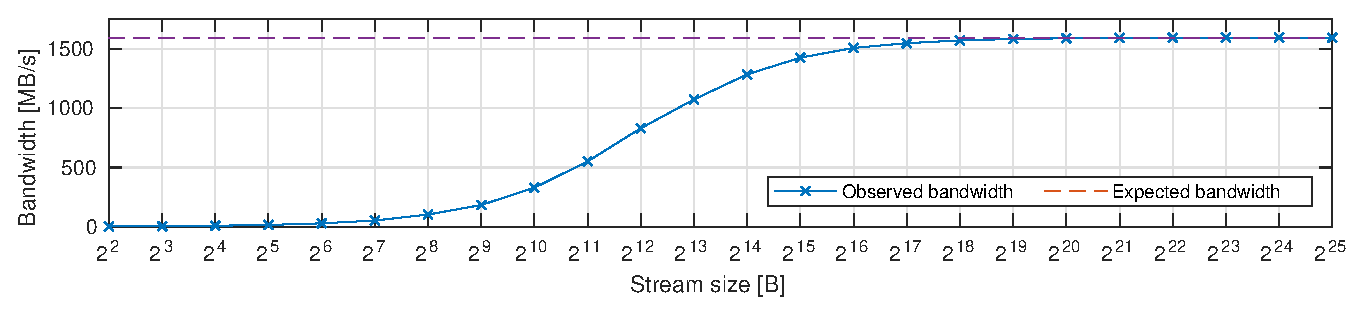
\includegraphics[width=\linewidth]{figures/xilinx_var_stream_size.eps}
    \caption{Observed duplex bandwidth for different stream sizes. The system was designed using a single 64-bit \ac{HP} port and a loop-back \ac{FIFO}, allowing to fully exploit the duplex bandwidth of the \ac{HP} port. The \ac{PL} operation frequency is \SI{100}{\mega\hertz}. Each data point represents the average of 200 transactions of the same size. The maximum standard deviation was \SI{5.70}{\mega\byte\per\second}.}
    \label{fig:xilinx_results_var_size}
\end{figure}

\begin{table}[!b]
\centering
\caption{Expected and observed bandwidth and respective system efficiency for several system configurations using \ac{HP} ports of the ZYNQ-7010 device. Each configuration was tested 200 times for \SI{32}{\mebi\byte} data blocks. The \ac{PL} operating frequency was \SI{100}{\mega\hertz}.}
\label{tab:xilinx_results_regular}
\begin{tabular}{cl|c|r|r|r|r|r|r|}
\cline{3-9}
\multicolumn{1}{l}{}                                                                  &                                                                          &                                            & \multicolumn{5}{c|}{\textbf{Bandwidth [\si{\mega\byte\per\second}]}}                                                                                                                                                      & \multicolumn{1}{c|}{}                                           \\ \cline{4-8}
\multicolumn{1}{l}{}                                                                  &                                                                          &                                            & \multicolumn{1}{c|}{}                                    & \multicolumn{4}{c|}{\textbf{Observed}}                                                                                                                         & \multicolumn{1}{c|}{}                                           \\ \cline{5-8}
\multicolumn{1}{l}{}                                                                  &                                                                          & \multirow{-3}{*}{\textbf{Channels}}        & \multicolumn{1}{c|}{\multirow{-2}{*}{\textbf{Expected}}} & \multicolumn{1}{c|}{\textbf{Average}} & \multicolumn{1}{c|}{\textbf{Minimum}} & \multicolumn{1}{c|}{\textbf{Maximum}} & \multicolumn{1}{c|}{$\mathbf{\sigma}$} & \multicolumn{1}{c|}{\multirow{-3}{*}{\textbf{Efficiency [\%]}}} \\ \hline
\multicolumn{1}{|c|}{}                                                                &                                                                          & \textbf{HP0}                               & 800.00                                                   & 799.95                                & 799.95                                & 799.96                                & 0.0003                                 & 99.99                                                           \\ \cline{3-9} 
\multicolumn{1}{|c|}{}                                                                &                                                                          & \textbf{HP0,1}                             & 1600.00                                                  & 1599.84                               & 1599.84                               & 1599.85                               & 0.0017                                 & 99.99                                                           \\ \cline{3-9} 
\multicolumn{1}{|c|}{}                                                                &                                                                          & \textbf{HP0,2}                             & 1600.00                                                  & 1599.83                               & 1599.79                               & 1599.84                               & 0.0085                                 & 99.99                                                           \\ \cline{3-9} 
\multicolumn{1}{|c|}{}                                                                &                                                                          & \cellcolor[HTML]{FFFF00}\textbf{HP0,1,2}   & \cellcolor[HTML]{FFFF00}2400.00                          & \cellcolor[HTML]{FFFF00}2288.49       & \cellcolor[HTML]{FFFF00}2280.15       & \cellcolor[HTML]{FFFF00}2293.17       & \cellcolor[HTML]{FFFF00}1.2566         & \cellcolor[HTML]{FFFF00}95.35                                   \\ \cline{3-9} 
\multicolumn{1}{|c|}{}                                                                & \multirow{-5}{*}{\textbf{\rotatebox{90}{Duplex}}}                        & \cellcolor[HTML]{FFFF00}\textbf{HP0,1,2,3} & \cellcolor[HTML]{FFFF00}3200.00                          & \cellcolor[HTML]{FFFF00}2773.13       & \cellcolor[HTML]{FFFF00}2697.44       & \cellcolor[HTML]{FFFF00}2789.70       & \cellcolor[HTML]{FFFF00}15.0109        & \cellcolor[HTML]{FFFF00}86.66                                   \\ \cline{2-9} 
\multicolumn{1}{|c|}{}                                                                &                                                                          & \textbf{HP0}                               & 400.00                                                   & 399.99                                & 399.99                                & 399.99                                & 0.0001                                 & 100.00                                                          \\ \cline{3-9} 
\multicolumn{1}{|c|}{}                                                                &                                                                          & \textbf{HP0,1}                             & 800.00                                                   & 799.96                                & 799.96                                & 799.96                                & 0.0006                                 & 100.00                                                          \\ \cline{3-9} 
\multicolumn{1}{|c|}{}                                                                &                                                                          & \textbf{HP0,2}                             & 800.00                                                   & 799.96                                & 799.96                                & 799.96                                & 0.0006                                 & 100.00                                                          \\ \cline{3-9} 
\multicolumn{1}{|c|}{}                                                                &                                                                          & \textbf{HP0,1,2}                           & 1200.00                                                  & 1199.91                               & 1199.91                               & 1199.92                               & 0.0010                                 & 99.99                                                           \\ \cline{3-9} 
\multicolumn{1}{|c|}{}                                                                & \multirow{-5}{*}{\textbf{\rotatebox{90}{PS to PL}}}                      & \textbf{HP0,1,2,3}                         & 1600.00                                                  & 1599.85                               & 1599.85                               & 1599.8521                             & 0.0002                                 & 99.99                                                           \\ \cline{2-9} 
\multicolumn{1}{|c|}{}                                                                &                                                                          & \textbf{HP0}                               & 400.00                                                   & 399.99                                & 399.99                                & 400.0000                              & 0.0078                                 & 100.00                                                          \\ \cline{3-9} 
\multicolumn{1}{|c|}{}                                                                &                                                                          & \textbf{HP0,1}                             & 800.00                                                   & 799.98                                & 799.96                                & 800.0000                              & 0.0229                                 & 100.00                                                          \\ \cline{3-9} 
\multicolumn{1}{|c|}{}                                                                &                                                                          & \textbf{HP0,2}                             & 800.00                                                   & 799.98                                & 799.96                                & 800.0000                              & 0.0228                                 & 100.00                                                          \\ \cline{3-9} 
\multicolumn{1}{|c|}{}                                                                &                                                                          & \textbf{HP0,1,2}                           & 1200.00                                                  & 1199.95                               & 1199.91                               & 1200.0000                             & 0.0493                                 & 100.00                                                          \\ \cline{3-9} 
\multicolumn{1}{|c|}{\multirow{-15}{*}{\textbf{\rotatebox{90}{32 bit per channel}}}} & \multirow{-5}{*}{\textbf{\rotatebox{90}{PL to PS}}}                      & \textbf{HP0,1,2,3}                         & 1600.00                                                  & 1599.92                               & 1599.85                               & 1600.0000                             & 0.0800                                 & 100.00                                                          \\ \hline\hline
\multicolumn{1}{|c|}{}                                                                & \multicolumn{1}{c|}{}                                                    & \textbf{HP0}                               & 1600.00                                                  & 1599.82                               & 1599.81                               & 1599.82                               & 0.0054                                 & 99.99                                                           \\ \cline{3-9} 
\multicolumn{1}{|c|}{}                                                                & \multicolumn{1}{c|}{}                                                    & \cellcolor[HTML]{FFFF00}\textbf{HP0,1}     & \cellcolor[HTML]{FFFF00}3200.00                          & \cellcolor[HTML]{FFFF00}2236.12       & \cellcolor[HTML]{FFFF00}2212.38       & \cellcolor[HTML]{FFFF00}2267.40       & \cellcolor[HTML]{FFFF00}6.3216         & \cellcolor[HTML]{FFFF00}69.88                                   \\ \cline{3-9} 
\multicolumn{1}{|c|}{}                                                                & \multicolumn{1}{c|}{}                                                    & \textbf{HP0,2}                             & 3200.00                                                  & 3197.63                               & 3193.18                               & 3198.68                               & 0.8462                                 & 99.93                                                           \\ \cline{3-9} 
\multicolumn{1}{|c|}{}                                                                & \multicolumn{1}{c|}{}                                                    & \cellcolor[HTML]{FFFF00}\textbf{HP0,1,2}   & \cellcolor[HTML]{FFFF00}4264.00                          & \cellcolor[HTML]{FFFF00}2659.35       & \cellcolor[HTML]{FFFF00}2639.86       & \cellcolor[HTML]{FFFF00}2682.41       & \cellcolor[HTML]{FFFF00}4.1705         & \cellcolor[HTML]{FFFF00}62.37                                   \\ \cline{3-9} 
\multicolumn{1}{|c|}{}                                                                & \multicolumn{1}{c|}{\multirow{-5}{*}{\textbf{\rotatebox{90}{Duplex}}}}   & \cellcolor[HTML]{FFFF00}\textbf{HP0,1,2,3} & \cellcolor[HTML]{FFFF00}4264.00                          & \cellcolor[HTML]{FFFF00}2675.65       & \cellcolor[HTML]{FFFF00}2108.10       & \cellcolor[HTML]{FFFF00}2969.61       & \cellcolor[HTML]{FFFF00}297.1049       & \cellcolor[HTML]{FFFF00}62.75                                   \\ \cline{2-9} 
\multicolumn{1}{|c|}{}                                                                & \multicolumn{1}{c|}{}                                                    & \textbf{HP0}                               & 800.00                                                   & 799.96                                & 799.95                                & 799.96                                & 0.0012                                 & 99.99                                                           \\ \cline{3-9} 
\multicolumn{1}{|c|}{}                                                                & \multicolumn{1}{c|}{}                                                    & \textbf{HP0,1}                             & 1600.00                                                  & 1599.84                               & 1599.83                               & 1599.84                               & 0.0018                                 & 99.99                                                           \\ \cline{3-9} 
\multicolumn{1}{|c|}{}                                                                & \multicolumn{1}{c|}{}                                                    & \textbf{HP0,2}                             & 1600.00                                                  & 1599.84                               & 1599.83                               & 1599.85                               & 0.0016                                 & 99.99                                                           \\ \cline{3-9} 
\multicolumn{1}{|c|}{}                                                                & \multicolumn{1}{c|}{}                                                    & \textbf{HP0,1,2}                           & 2400.00                                                  & 2399.66                               & 2399.64                               & 2399.66                               & 0.0054                                 & 99.99                                                           \\ \cline{3-9} 
\multicolumn{1}{|c|}{}                                                                & \multicolumn{1}{c|}{\multirow{-5}{*}{\textbf{\rotatebox{90}{PS to PL}}}} & \textbf{HP0,1,2,3}                         & 3200.00                                                  & 3184.87                               & 3103.57                               & 3199.38                               & 16.7246                                & 99.53                                                           \\ \cline{2-9} 
\multicolumn{1}{|c|}{}                                                                & \multicolumn{1}{c|}{}                                                    & \textbf{HP0}                               & 800.00                                                   & 799.98                                & 799.95                                & 800.00                                & 0.0286                                 & 100.00                                                          \\ \cline{3-9} 
\multicolumn{1}{|c|}{}                                                                & \multicolumn{1}{c|}{}                                                    & \textbf{HP0,1}                             & 1600.00                                                  & 1599.91                               & 1599.83                               & 1600.00                               & 0.0917                                 & 99.99                                                           \\ \cline{3-9} 
\multicolumn{1}{|c|}{}                                                                & \multicolumn{1}{c|}{}                                                    & \textbf{HP0,2}                             & 1600.00                                                  & 1599.91                               & 1599.83                               & 1600.00                               & 0.0914                                 & 100.00                                                          \\ \cline{3-9} 
\multicolumn{1}{|c|}{}                                                                & \multicolumn{1}{c|}{}                                                    & \textbf{HP0,1,2}                           & 2400.00                                                  & 2399.83                               & 2399.63                               & 2400.00                               & 0.1895                                 & 99.99                                                           \\ \cline{3-9} 
\multicolumn{1}{|c|}{\multirow{-15}{*}{\textbf{\rotatebox{90}{64 bit per channel}}}} & \multicolumn{1}{c|}{\multirow{-5}{*}{\textbf{\rotatebox{90}{PL to PS}}}} & \textbf{HP0,1,2,3}                         & 3200.00                                                  & 3199.70                               & 3199.39                               & 3200.00                               & 0.3170                                 & 99.99                                                           \\ \hline
\end{tabular}
\end{table} %

Although the previous experiments allowed to fully exploit the bandwidth of the on-chip high-performance interfaces in duplex mode, they were insufficient to reproduce the results obtained by G{\"{o}}bel \textit{et al.} regarding the \ac{PS}-to-\ac{PL} bandwidth of the Xilinx device. In order to increase even further the bandwidth requirement on the \ac{PL} side, the system to evaluate the \ac{PS}-to-\ac{PL} bandwidth was re-implemented for an operating frequency of \SI{150}{\mega\hertz}. With the new operation frequency, the \ac{PL} component of the system is capable of a maximum data rate of \SI{4800}{\mega\byte\per\second}, which is even higher than the DDR maximum bandwidth. The results of this experiment are shown in Table \ref{tab:results_xilinx_stress_150}. As expected, the maximum achieved bandwidth surpasses that of the same system implemented for an operating frequency of \SI{100}{MHz}. The configuration that leads, in average, to the highest data rate (\SI{3448.33}{\mega\byte\per\second}) is the one using \ac{HP} ports 0, 1 and 2. The maximum achieved data rate is compatible with the conclusions of G{\"{o}}bel \textit{et al.} Furthermore, in one or more experiments using all the four \ac{HP} ports, a bandwidth higher than \SI{4}{\giga\byte\per\second} was obtained. However, such performance is not always possible due to limitations at the memory controller level. It is also worth mentioning that, under stress, the \ac{HP} ports achieve higher data rates on single-sided transfers than on duplex transfers.

\begin{table}[!b]
\centering
\caption{Expected and observed bandwidth and respective system efficiency for configurations aiming at exploiting the maximum \ac{PS}-to-\ac{PL} bandwidth. Each configuration was tested 200 times for \SI{32}{\mebi\byte} data blocks. The \ac{PL} operating frequency was \SI{150}{\mega\hertz}.}
\label{tab:results_xilinx_stress_150}
\begin{tabular}{c|c|r|r|r|r|r|r|}
\cline{2-8}
                                                                                                                    &                                            & \multicolumn{5}{c|}{\textbf{Bandwidth [\si{\mega\byte\per\second}]}}                                                                                                                                                      & \multicolumn{1}{c|}{}                                           \\ \cline{3-7}
                                                                                                                    &                                            & \multicolumn{1}{c|}{}                                    & \multicolumn{4}{c|}{\textbf{Observed}}                                                                                                                         & \multicolumn{1}{c|}{}                                           \\ \cline{4-7}
                                                                                                                    & \multirow{-3}{*}{\textbf{Channels}}        & \multicolumn{1}{c|}{\multirow{-2}{*}{\textbf{Expected}}} & \multicolumn{1}{c|}{\textbf{Average}} & \multicolumn{1}{c|}{\textbf{Minimum}} & \multicolumn{1}{c|}{\textbf{Maximum}} & \multicolumn{1}{c|}{$\mathbf{\sigma}$} & \multicolumn{1}{c|}{\multirow{-3}{*}{\textbf{Efficiency [\%]}}} \\ \hline
\multicolumn{1}{|c|}{}                                                                                              & \textbf{HP0}                               & 1200                                                     & 1199.91                               & 1199.91                               & 1199.91                               & 0.0005                                 & 99.99                                                           \\ \cline{2-8} 
\multicolumn{1}{|c|}{}                                                                                              & \textbf{HP0,1}                             & 2400                                                     & 2393.39                               & 2371.02                               & 2397.02                               & 2.3698                                 & 99.72                                                           \\ \cline{2-8} 
\multicolumn{1}{|c|}{}                                                                                              & \textbf{HP0,2}                             & 2400                                                     & 2396.52                               & 2396.07                               & 2398.13                               & 0.2730                                 & 99.86                                                           \\ \cline{2-8} 
\multicolumn{1}{|c|}{}                                                                                              & \cellcolor[HTML]{FFFF00}\textbf{HP0,1,2}   & \cellcolor[HTML]{FFFF00}3600                             & \cellcolor[HTML]{FFFF00}3448.33       & \cellcolor[HTML]{FFFF00}3413.08       & \cellcolor[HTML]{FFFF00}3510.90       & \cellcolor[HTML]{FFFF00}11.2324        & \cellcolor[HTML]{FFFF00}95.79                                   \\ \cline{2-8} 
\multicolumn{1}{|c|}{\multirow{-5}{*}{\textbf{\begin{tabular}[c]{@{}c@{}}64 bit/\\ channel,\\ PS to PL\end{tabular}}}} & \cellcolor[HTML]{FFFF00}\textbf{HP0,1,2,3} & \cellcolor[HTML]{FFFF00}4264                             & \cellcolor[HTML]{FFFF00}3154.97       & \cellcolor[HTML]{FFFF00}2939.33       & \cellcolor[HTML]{FFFF00}4001.69       & \cellcolor[HTML]{FFFF00}133.1674       & \cellcolor[HTML]{FFFF00}73.99                                   \\ \hline
\end{tabular}
\end{table} %

To conclude the assessment of the ZYNQ-7000 device, another scenario based on the system to evaluate the duplex bandwidth was considered in which streams of multiple sizes were transferred from the \ac{PS} to the \ac{PL} and back to the \ac{PS}. For this experiment, a single 64-bit \ac{HP} port was used, the \ac{PL} operation frequency was set to \SI{100}{\mega\hertz}, and each stream size was tested 200 times. Figure \ref{fig:xilinx_results_var_size} illustrates the results of this experiment. Results show that small stream sizes only achieve a fraction of the theoretical maximum bandwidth allowed by the used configuration. Only for streams bigger than \SI{64}{\kibi\byte} a real bandwidth of more than 90\% of the theoretical maximum is achieved.

%\clearpage